\documentclass[12pt,letterpaper,titlepage]{article}

\usepackage{fontspec}
\defaultfontfeatures{Mapping=tex-text}
\usepackage{xunicode}
\usepackage{xltxtra}
\usepackage{amsmath}
\usepackage{pdfpages}
\usepackage{amsfonts}
\usepackage{bbold}
\usepackage{amssymb}
\setcounter{secnumdepth}{0}
\usepackage{nameref}
\usepackage{enumitem}
\usepackage{environ}
\usepackage{pgfplots}
\usepackage{listings}

\showboxdepth=\maxdimen
\showboxbreadth=\maxdimen


\usepackage{paracol}
\usepackage{wrapfig}
\globalcounter{table}
\globalcounter{figure}
\usepackage{graphicx}
\usepackage[left=1in,right=1in,top=1in,bottom=1in]{geometry}
\graphicspath{{img/}}

\author{Jacob Abel}
\title{	Design \& Simulate 26
	\\\large ECE2204 CRN:82929
}

\setlength{\parskip}{0.5em}

\begin{document}
\maketitle
\begin{raggedright}
\section{Problem 21.16-11.a.1: } 
\subsection{Design}



\begin{center}
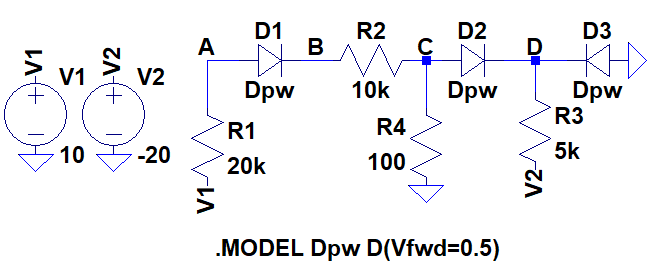
\includegraphics[width=\textwidth, height=25\baselineskip, keepaspectratio=true]{ds1}
\end{center}

\clearpage
\subsection{Validation}

\begin{center}
LTSpice Implementation (All values of truth table match waveform)
\columnratio{0.65}
\begin{paracol}{2}
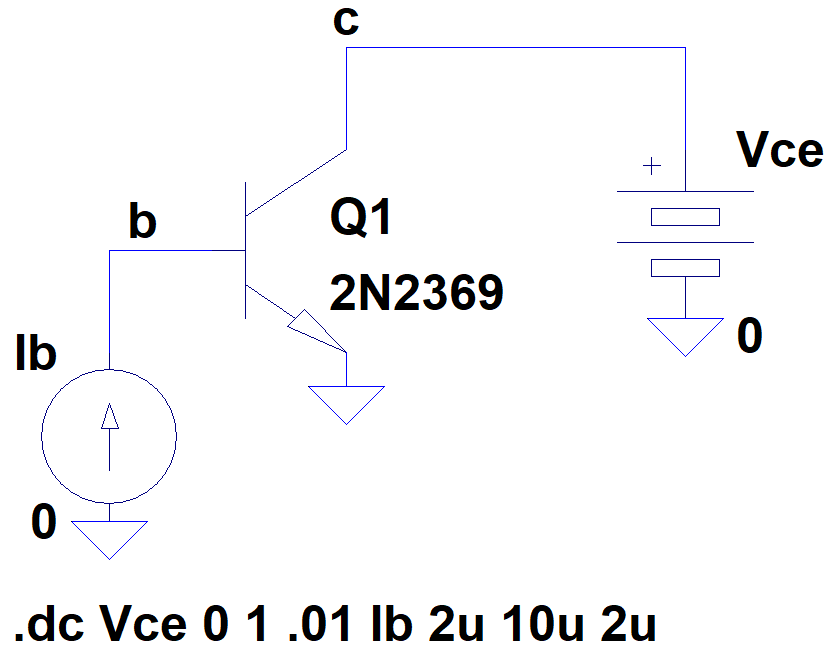
\includegraphics[width=0.64\textwidth, height=\textheight, keepaspectratio=true]{ds1b}
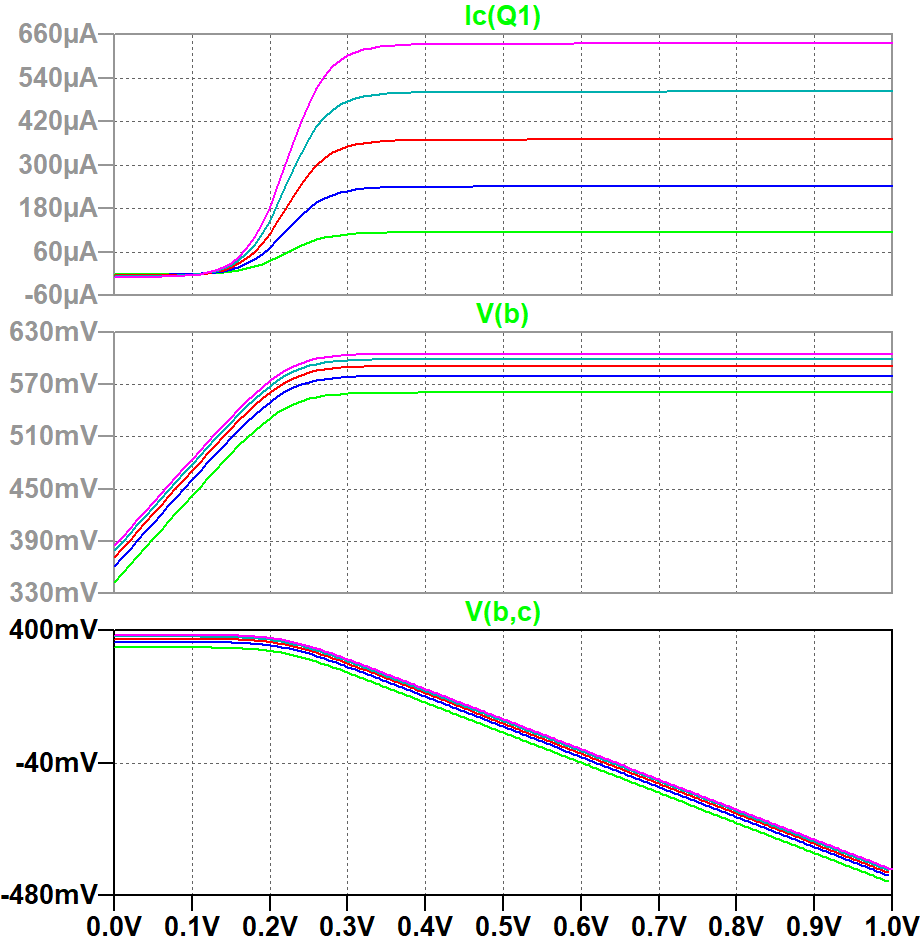
\includegraphics[width=0.64\textwidth, height=\textheight, keepaspectratio=true]{ds1c}
\switchcolumn
\begin{tabular}{| c | l |}
  \hline ABCDE & F(A,B,C,D,E)
\\\hline 00000 & 1
\\\hline 00001 & 1
\\\hline 00010 & 1
\\\hline 00011 & 1
\\\hline 00100 & 1
\\\hline 00101 & 1
\\\hline 00110 & 1
\\\hline 00111 & 0
\\\hline 01000 & 1
\\\hline 01001 & 1
\\\hline 01010 & 1
\\\hline 01011 & 1
\\\hline 01100 & 1
\\\hline 01101 & 1
\\\hline 01110 & 1
\\\hline 01111 & 0
\\\hline 10000 & 1
\\\hline 10001 & 0
\\\hline 10010 & 1
\\\hline 10011 & 0
\\\hline 10100 & 1
\\\hline 10101 & 0
\\\hline 10110 & 1
\\\hline 10111 & 0
\\\hline 11000 & 0
\\\hline 11001 & 0
\\\hline 11010 & 0
\\\hline 11011 & 0
\\\hline 11100 & 0
\\\hline 11101 & 0
\\\hline 11110 & 0
\\\hline 11111 & 0
\\\hline
\end{tabular}
\end{paracol}
\end{center}

This problem should demonstrate a basic ability to manipulate, design, and analyse MOSFET based logic circuits. 

\textit{I have neither given nor received unauthorized assistance on this assignment.}


\end{raggedright}
\end{document}
